\documentclass[letterpaper]{article}
\usepackage{aaai}
\usepackage{times}
\usepackage{algorithm}
\usepackage{algpseudocode}
\usepackage{subfigure}
\usepackage{graphicx}
\usepackage{subfloat}
\usepackage{float}
\usepackage{mathtools}% http://ctan.org/pkg/mathtools
\usepackage{amsmath,empheq}
\usepackage{amssymb}
\usepackage{latexsym}
\usepackage{booktabs}
\usepackage[numbers]{natbib}
\usepackage{multicol}
\usepackage[bookmarks=true]{hyperref}
\usepackage[usenames,dvipsnames]{color}
\usepackage{tikz}
\usepackage{pgfplots}
\usepackage[scientific-notation=true]{siunitx}

% -- Comment commands --
 \newcommand{\stnote}[1]{\textcolor{Blue}{\textbf{stefie10: #1}}}
 \newcommand{\dnote}[1]{\textcolor{Green}{\textbf{dabel:  #1}}}
 \newcommand{\enote}[1]{\textcolor{Red}{\textbf{ellis:  #1}}}
 \newcommand{\gnote}[1]{\textcolor{Purple}{\textbf{gabe:  #1}}}
 \newcommand{\jnote}[1]{\textcolor{Orange}{\textbf{james:  #1}}}
%	\raggedbottom

% -- Misc. new commands --
\newcommand{\argmax}{\operatornamewithlimits{argmax}} % argmax
\newcommand{\ra}[1]{\renewcommand{\arraystretch}{#1}} % booktabs table cmd

\begin{document}

% paper title
\title{Goal-Based Action Priors}

% Author info:
\author{David Abel, D. Ellis Hershkowitz, Gabriel Barth-Maron, \\ {\Large {\bf Stephen Brawner, Kevin O'Farrell, James MacGlashan, Stefanie Tellex}}\\
Brown University, Computer Science Department\\
115 Waterman Street, 4th floor
Providence, RI 02912
}


\maketitle

\begin{abstract}
Robots that interact with people must flexibly respond to
requests by planning in stochastic state spaces that are often too large to solve for optimal behavior.
In this work, we develop a framework for goal and state dependent
action priors that can be used to prune away irrelevant actions based on the
robot's current goal, thereby greatly accelerating planning in a variety of
complex stochastic environments. Our framework allows these goal-based action priors to be
specified by an expert or to be learned from prior experience in related
problems. We evaluate our approach in the video game Minecraft, whose complexity
makes it an effective robot simulator. We also evaluate our approach in a robot cooking domain that
is executed on a two-handed manipulator robot. In both cases, goal-based action priors enhance
baseline planners by dramatically reducing the time taken to find a near-optimal plan.
\end{abstract}

%\maketitle

% ====== Section: Introduction ======
\section{Introduction}
\label{sec:introduction}

Robots operating in unstructured, stochastic environments such as a
factory floor or a kitchen face a difficult planning problem due to
the large state space and the very large set of possible
tasks~\citep{bollini12,knepper13}.  A powerful and flexible robot such
as a mobile manipulator in the home has a very large set of possible
actions, any of which may be relevant depending on the current goal
(for example, robots assembling furniture~\citep{knepper13} or baking
cookies~\citep{bollini12}.) When a robot is manipulating objects in
an environment, an object can be placed anywhere in a large set of
locations.  The size of the state space increases exponentially with
the number of objects, which bounds the placement problems that the
robot is able to expediently solve.  Depending on the reward function
(which is unknown before runtime), any of these states and actions may
be relevant to the solution, but for any specific reward function,
most of them are irrelevant.  For instance, when making brownies, the
oven and flour are important, while the soy sauce and saut\'{e} pan
are not.  For a different task, such as stir-frying broccoli, the
robot must use a different set of objects and
actions. 

Robotic planning tasks are often formalized as a stochastic sequential
decision making problem, modeled as a Markov Decision Process
(MDP)~\citep{thrun2008probabilistic}. In these problems, the agent
must find a mapping from states to actions for some subset of the
state space that enables the agent to achieve a goal while minimizing
costs along the way.  However, many robotics problems correspond to a
family of related MDPs; following STRIPs terminology, these problems
come from the same domain, but each task may have a different reward
function or goal condition.  For example, figure~\ref{fig:example}
shows an example of two problems from the same domain in the game
Minecraft~\citep{minecraft}.

%\begin{figure}
%\centering
%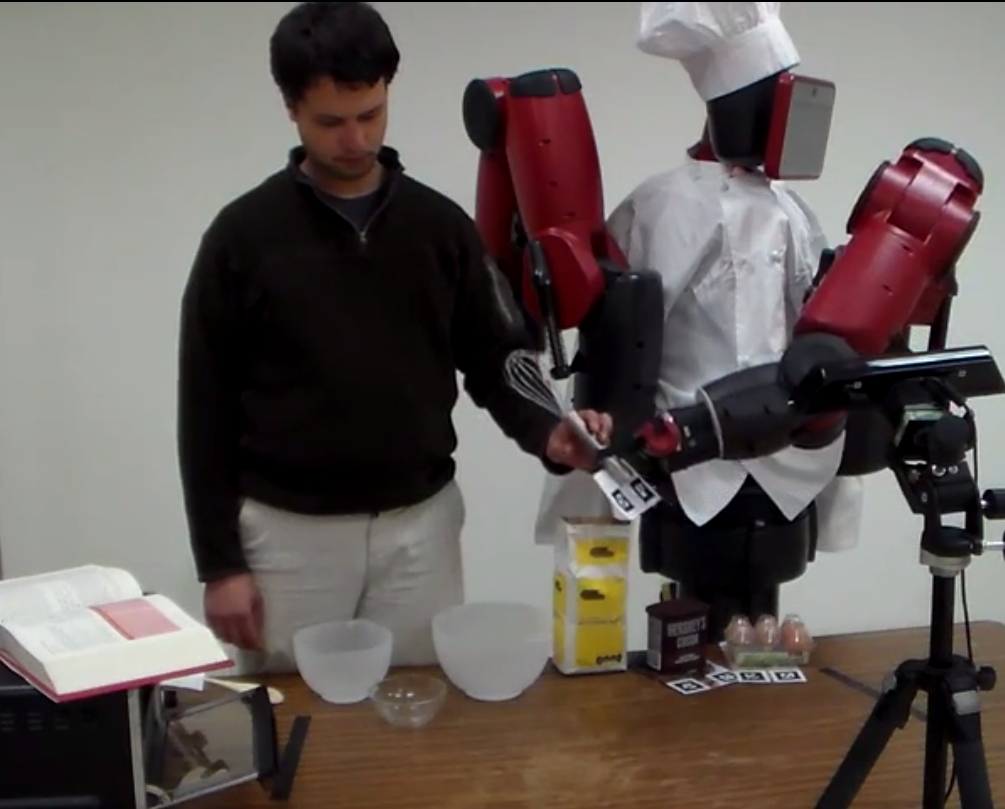
\includegraphics[width=0.75\linewidth]{figures/baxter.png}%
%  \caption{Affordances enable a robot to efficiently infer helpful actions in
%    very large state spaces, such as a kitchen.}
%  \label{fig:baxter_results}
%\end{figure}

\begin{figure}
\centering
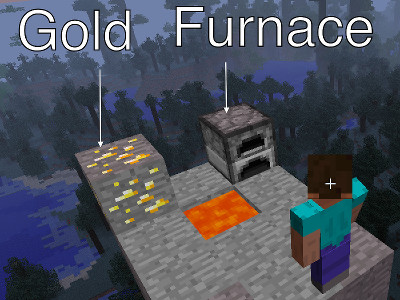
\includegraphics[width=0.49\linewidth]{figures/smelt_small.jpg}
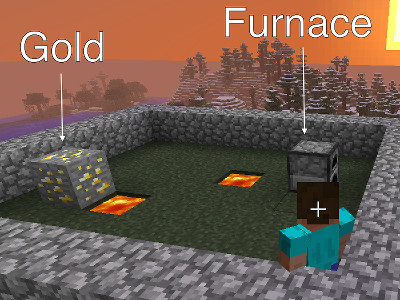
\includegraphics[width=0.49\linewidth]{figures/smelt_large.jpg}
\caption{Two different problems from the same domain, where the
  agent's goal is to smelt the gold in the furnace while avoiding the
  lava.  Our agent is unable to solve the problem on the right before
  learning because the state/action space is too large (since it can
  place the gold block anywhere).  After learning, it can quickly
  solve the larger problem.\label{fig:example}}
\end{figure}


To confront this state-action space explosion, prior work has explored
adding knowledge to the planner, such as options~\cite{sutton99} and
macro-actions~\cite{Botea:2005kx,Newton:2005vn}.  However, while these
methods can allow the agent to search more deeply in the state space,
they add non-primitive actions to the planner which {\em increase} the
branching factor of the state-action space.  The resulting augmented
space is even larger, which can have the paradoxical effect of
increasing the search time for a good policy~\cite{Jong:2008zr}.
Deterministic forward-search algorithms like hierarchical task
networks (HTNs)~\citep{Nau:1999:SSH:1624312.1624357}, and temporal
logical planning
(TLPlan)~\citep{Bacchus95usingtemporal,Bacchus99usingtemporal}, add
knowledge to the planner that greatly increases planning speed, but do
not generalize to stochastic domains. Additionally, the knowledge
provided to the planner by these methods is quite extensive, reducing
the agent's autonomy.

To address these issues, we augment an Object Oriented Markov Decision
Process (OO-MDP) with a specific type of action prior conditioned on
the current state and an abstract goal description. This {\it goal-based action prior}
enables the robot to prune irrelevant actions on a
state-by-state basis according to the agent's current goal, focusing the robot on
the most promising parts of the state space.  

Because we condition on
both the state and goal description, we note that there is a strong connection to the notion of an {\em affordance}.
Affordances were originally proposed by \citet{gibson77} as action possibilities
prescribed by an agent's capabilities in an environment. \stnote{Talk
  about Chemmaro here.}  
  
  Our goal-based action priors can be specified
by hand or alternatively learned through experience in related
problems, making them a concise, transferable, and learnable means of
representing useful planning knowledge. Our experiments demonstrate
that these priors provide dramatic improvements for a variety of
planning tasks compared to baselines in simulation, and are applicable
across different tasks.  Moreover, while manually provided
priors outperform baselines, priors learned through
experience yield even greater improvements.  We conduct experiments in
the video game Minecraft, which has a very large state-action space, and on
a real-world robotic cooking assistant.  Figure~\ref{fig:example}
shows an example of two problems from the same domain in the game
Minecraft; the agent learns on randomly generated problems and tests
on new problems from the same domain that it has never previously
encountered.  All associated code with this paper may be found at
\url{http://h2r.cs.brown.edu/affordances}.  \stnote{Make this link
  real.}

% ====== Section: Related Work ======
% ====== Affordances ======
\section{Technical Approach}
\label{sec:affordances}

We define goal-based action priors as formal knowledge added to a family of related
Markov Decision Processes (MDP) from the same domain.  An MDP is a
five-tuple: $\langle \mathcal{S}, \mathcal{A}, \mathcal{T},
\mathcal{R}, \gamma \rangle$, where $\mathcal{S}$ is a state space;
$\mathcal{A}$ is the agent's set of actions; $\mathcal{T}$ denotes
$\mathcal{T}(s' \mid s,a)$, the transition probability of an agent
applying action $a \in \mathcal{A}$ in state $s \in \mathcal{S}$ and
arriving in $s' \in \mathcal{S}$; $\mathcal{R}(s,a,s')$ denotes the
reward received by the agent for applying action $a$ in state $s$ and
transitioning to state $s'$; and $\gamma \in [0, 1)$ is a discount
  factor that defines how much the agent prefers immediate rewards
  over future rewards (the agent prefers to maximize immediate rewards
  as $\gamma$ decreases). 

Our priors build on Object-Oriented MDPs
(OO-MDPs)~\citep{diuk08}.  An OO-MDP efficiently represents the state
of an MDP through the use of objects and predicates.  An OO-MDP state
is a collection of objects, $O = \{o_1, \ldots, o_o \}$.  Each object
$o_i$ belongs to a class, $c_j \in \{c_1, \ldots, c_c\}$. Every class
has a set of attributes, $Att(c) = \{c.a_1, \ldots, c.a_a \}$, each of
which has a domain, $Dom(c.a)$, of possible values. OO-MDPs enable
planners to use predicates over classes of objects. That is, the
OO-MDP definition also includes a set of predicates $\mathcal{P}$ that
operate on the state of objects to provide additional high-level
information about the MDP state.


\begin{figure}
\subfigure[Domain]{
\fbox{
\parbox{0.47\linewidth}{\tiny
\begin{itemize}
  \item Object Classes:
    \begin{itemize}
    \item Agent
      \begin{itemize}
      \item Location (x, y, z)
      \item Inventory
      \end{itemize}
    \item Block
      \begin{itemize}
      \item Type (Wood, Lava, ...)
      \item Location (x, y, z)
      \item Destructible (True, False)
%      \item LeavesItemBehind (True, False)
      \end{itemize}
    \end{itemize}
  \item Actions: {\sf DestroyBlock}, {\sf UseBlock}, {\sf TurnLeft},
    {\sf TurnRight}, {\sf MoveForward}, {\sf LookUp}, {\sf LookDown}, {\sf PlaceBlock}, {\sf Jump}
  \item Transition Dynamics: Movement actions (Look, Turn, Move) incorrectly apply a different move action 5\% of the time. % This was done because effectively "null" action applications are uninteresting and do not affect planning at all (presence of lava is irrelevant). With this style, if we are facing lava and try to turn away, we might walk into it.
    \end{itemize}
}}}%
\subfigure[Example tasks.]{
  \fbox{\parbox{0.47\linewidth}{\tiny
Agent is standing at (x, y, z).\\
Agent has smelted gold.\\
Agent has acquired ore.\\
Agent has constructed a tower of height K.\\
Agent has built a cube with edge length K.\\
Agent has destroyed K blocks.\\
}}
}
\caption{Part of the OO-MDP Domain for the Minecraft.\label{fig:oomdp}}
\end{figure}

OO-MDP predicates provide state space independence. For a given
planning domain, OO-MDP objects often appear across tasks. Since
predicates operate on collections of objects, they generalize beyond
specific state spaces within the domain.  For instance, in Minecraft,
a predicate checking the contents of the agent's inventory generalizes
beyond any particular Minecraft task. We capitalize on this state
space independence by using OO-MDP predicates as features for action
pruning. Figure~\ref{fig:oomdp} shows part of the definition of our Minecraft domain, as well as
several example tasks in the Minecraft domain.

% -- Figure: Minecraft pic --
\begin{figure}[b]
\centering
\subfigure[Mine the gold and smelt it in the furnace]{
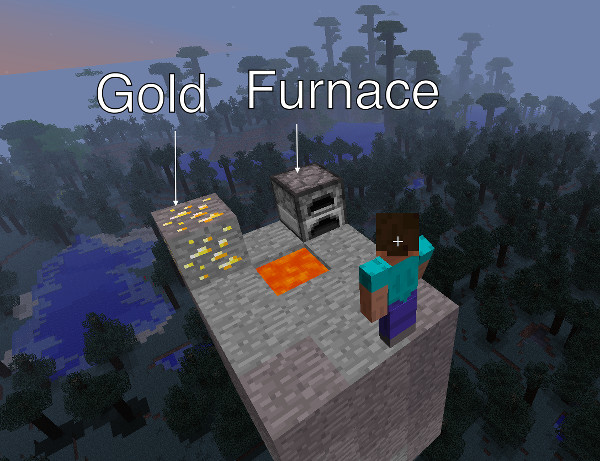
\includegraphics[width=0.3\linewidth]{figures/smelt_labeled_small.jpg}}
\subfigure[Dig down to the gold and mine it, avoiding lava.]{
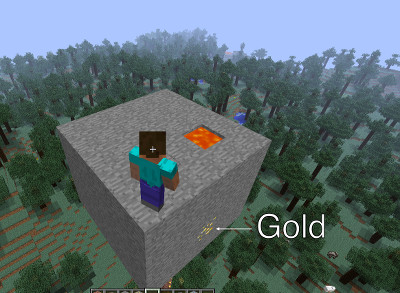
\includegraphics[width=0.3\linewidth]{figures/mining_labeled.jpg}}
\subfigure[Navigate to the goal location, avoiding lava.]{
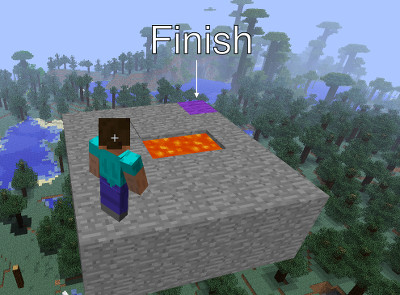
\includegraphics[width=0.3\linewidth]{figures/plane.jpg}}
  \caption{Three different problems from the Minecraft domain}
  \label{fig:minecraft}
\end{figure}

Following STRIPs terminology, we define a domain as a family of
related MDPs with the same state space, action space, and transition
dynamics, but different reward functions, terminal states, and initial
states.  Analogously, a
STRIPs problem is a specific MDP with a known reward function, set
of terminal states, and an initial state.  We are
concerned with MDPs where the reward function is goal-directed, that
is the agent receives a negative reward at each time step that motivates
it to reach the goal terminal state.  A goal, $G$ is
defined by a reward function plus a non-empty set of terminal states. The aim
of our approach is to learn knowledge about a domain from experience
that enables an agent to quickly infer a solution to a new problem in
the same domain that it has never previously encountered.


% -- Subsection: Modeling the Optimal Actions --
\subsection{Modeling the Optimal Actions}

Our goal is to formalize planning knowledge that allows an agent to
avoid searching suboptimal actions in each state based on the agent's
current goal. We define the optimal action set, $\mathcal{A}^*$, for a
given state $s$ and goal $G$ as:
% -- Equation: Optimal Action Set --
\begin{equation}
\mathcal{A}^* = \left\{ a \mid Q^*_G(s,a) = V^*_G(s) \right\}, 
\label{eq:opt_act_set}
\end{equation}
where $Q^*_G(s,a)$ and $V^*_G(s)$ represent the optimal Q function and 
value function, respectively.

We aim to learn a probability distribution over the optimality of each action
for a given state ($s$), goal ($G$). Thus, we want to infer a Bernoulli
distribution for each action's optimality:
% -- Equation: Master Equation --
\begin{equation}
\Pr(a_i \in \mathcal{A}^* \mid s, G)
\label{eq:master}
\end{equation}

\noindent for $i \in \{1, \ldots, |\mathcal{A}|\}$, where
$\mathcal{A}$ is the OO-MDP action space for the domain.

To generalize across specific low-level states, we abstract the state
and goal into a set of $n$ paired preconditions and goal types, $\{
(p_1, g_1) \ldots (p_{n}, g_{n}) \}$. We abbreviate each pair $(p_j,
g_j)$ to $\delta_j$ for simplicity. Each precondition $p \in
\mathcal{P}$ is a {\it predicate} in the set of predicates $\mathcal{P}$
defined by the OO-MDP domain, and $g$ is a {\it goal type} which is a
logical expression that defines a subset of goals. For example, a
predicate might be $nearTrench(agent)$ which is true when the agent is
standing near a trench.  In general a precondition is an arbitrary
logical expression of the state; in our experiments we used unary
predicates defined in the OO-MDP domain.  A goal type specifies the
sort of problem the agent is trying to solve, such as the agent
retrieving an object of a certain type from the environment, reaching
a particular location, or creating a new structure.  Depending on the
agent's current goal, the relevance of each action changes
dramatically.  We rewrite Equation~\ref{eq:master}:
% -- Equation: replace K --
\begin{multline}
\Pr(a_i \in \mathcal{A}^* \mid s, G)
= \Pr(a_i \in \mathcal{A}^* \mid \delta_1 \ldots \delta_n).
\end{multline}

We introduce the indicator function $f$, which returns 1 if and only if $\delta_j$'s predicate is true in the provided state $s$, and $\delta_j$'s goal type is entailed by the agent's current goal, $G$:
% -- Equation: function f defn --
\begin{equation}
f(\delta, s, G) = 
\begin{cases}
1& \delta.p(s) \wedge \delta.g(G) \\
0& \text{otherwise.}
\end{cases}
\label{eq:f_func_def}
\end{equation}

Evaluating $f$ for each $\delta_j$ given the current state and goal gives rise to a set of binary features,
$\phi_j = f(\delta_j, s, G)$, which we use to reformulate our probability distribution:
% -- Equation: replace deltas with phi --
\begin{multline}
\Pr(a_i \in \mathcal{A}^*  \mid s, G, \delta_1 \ldots \delta_n) \\
= \Pr(a_i \in \mathcal{A}^*  \mid \phi_1, \ldots, \phi_n)
\label{eq:feature_rep}
\end{multline}

This distribution may be modeled in a number of ways, making this
approach quite flexible. One model that can be easily specified by
an expert is an OR model.
In the OR model some subset of the features 
($\phi^i \subset \phi$) are
assumed to cause action $a_i$ to be optimal; as long as one of
the features is on, the probability that $a_i$ is optimal is one.
If none of the features are on, then the probability that $a_i$ is 
optimal is zero. More formally,
\begin{equation}
\Pr(a_i \in \mathcal{A}^*  \mid \phi_1, \ldots, \phi_n) = \phi_1^i \lor ... \lor \phi_m^i,
\end{equation}
where $m$ is the number of features that can cause $a_i$ to be optimal ($m = |\phi^i|$).

In practice, we do not expect such a distribution to be reflective of
reality; if it were, then no planning would be needed because a full
policy would have been specified. However, it does provide a
convenient way for a designer to provide conservative background
knowledge. Specifically, a designer can consider each precondition-goal
pair and specify the actions that could be optimal in that context, ruling
out actions that would be known to be irrelevant or dependent on other
state features being true. For example,
Table~\ref{table:afford_kb_exp} shows example expert-provided
conditions that we used in our Minecraft experiments.

Because the OR model is not expected to be reflective of
reality and because of other limitations (such as not allowing support
for an action to be provided when a feature is off), the model is not
practical for learning.  Learned priors have the potential to outperform
hand-coded priors by more flexibly adapting to the
features that predict optimal actions over a large training set.  An
alternative more expressive model that does lend itself to learning is
Naive Bayes. We first factor using Bayes' rule, introducing a parameter vector $\theta_i$ of
feature weights:

% -- Equation: Bayes --
\begin{equation}
= \frac{\Pr(\phi_1, \ldots, \phi_{n}, \mid a_i \in \mathcal{A}^*, \theta_i) \Pr(a_i \in \mathcal{A}^* \mid \theta_i)}{\Pr(\phi_1, \ldots, \phi_{n} | \theta_i)}
\label{eq:bayes}
\end{equation}

Next we assume that each feature is conditionally independent of the others, given whether the action is optimal:
% -- Equation: Naive assumption and uniform prior--
\begin{equation}
= \frac{\prod_{j=1}^{n} \Pr(\phi_j \mid a_i \in \mathcal{A}^*, \theta_i) \Pr(a_i \in \mathcal{A}^* \mid \theta_i) }{\Pr(\phi_1, \ldots, \phi_{n} | \theta_i)}
\label{eq:final}
\end{equation}

Finally, we define the prior on the optimality of each action to be
the fraction of the time each action was optimal during training.
%This approach allows model parameters to be learned from optimal
%policies during training, and information from different state
%precondition functions to be combined to infer a distribution on
%affordances.
Although we only explore hard affordance and Naive Bayes
models in this work, other affordance models, like logistic regression
and Noisy-Or, could also be used.




%In a recent review on the theory of affordances,~\citet{chemero2003}
%suggests that an affordance is a relation between the features of an
%environment and an agent's abilities. Our approach grounds this
%interpretation, where the features of the environment correspond to
%the goal-dependent state features, $\phi$, and the agent's abilities
%correspond to the OO-MDP action set.  We define an affordance, $A$, 
%\begin{align}
%A \equiv \left< \delta_j, Pr(a_i \in \mathcal{A}^* |
%\phi_j; \theta) \right>
%\end{align}
%We can compute this term in our Naive Bayes model by marginalizing
%over all the features not associated with $\phi_j$.  Alternatively,
%hard affordances may be specified by an expert by setting this
%distribution to zero or one. 


% -- Subsection: Learning the Optimal Actions--
\subsection{Learning the Optimal Actions}
Using the above model allows us to learn an action prior
through experience. We provide a set of
training worlds from the domain ($W$), for which the optimal policy,
$\pi$, may be tractably computed using existing planning methods.  We
compute model parameters using the small training worlds, and then
evaluate performance on a different set of much harder problems at
test time.  To compute model parameters using Naive Bayes, we compute
the maximum likelihood estimate of the parameter vector $\theta_i$ for
each action using the policy.

Under our Bernouli Naive Bayes model, we estimate the parameters
$\theta_{i,0} = \Pr(a_i)$ and $\theta_{i,j} = \Pr(\phi_j | a_i)$, for $j \in \{1, \ldots, n \}$, where the maximum likelihood estimates are:
\begin{align}
\theta_{i,0} &= \frac{C(a_i)}{C(a_i) + C(\bar{a_i})} \\
\theta_{i,j} &= \frac{C(\phi_j, a_i)}{C(a_i)}
\end{align}

\begin{figure}[H]
\centering
\subfigure[agentLookTowardGoal]{
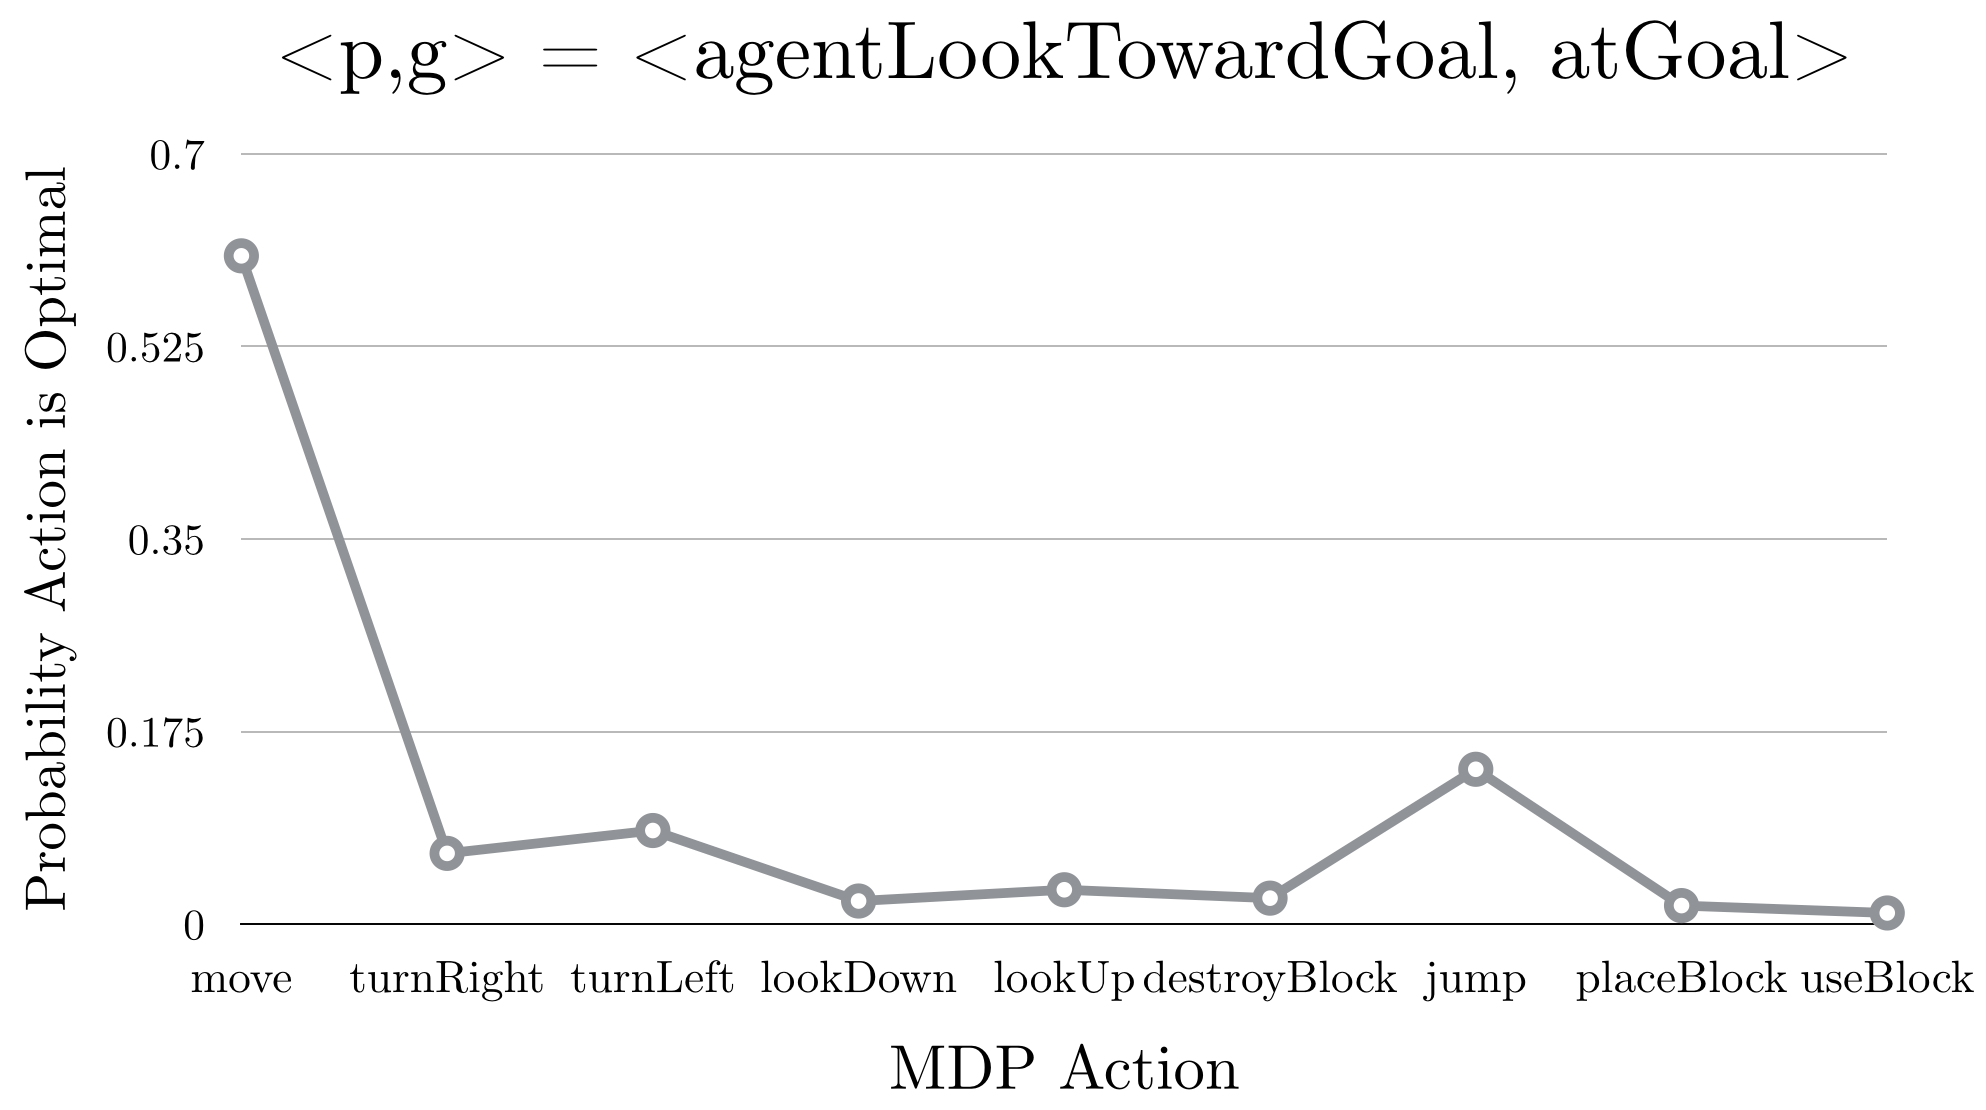
\includegraphics[scale=0.17]{figures/plane_aff.png}}
\subfigure[trenchInFrontOfAgent]{
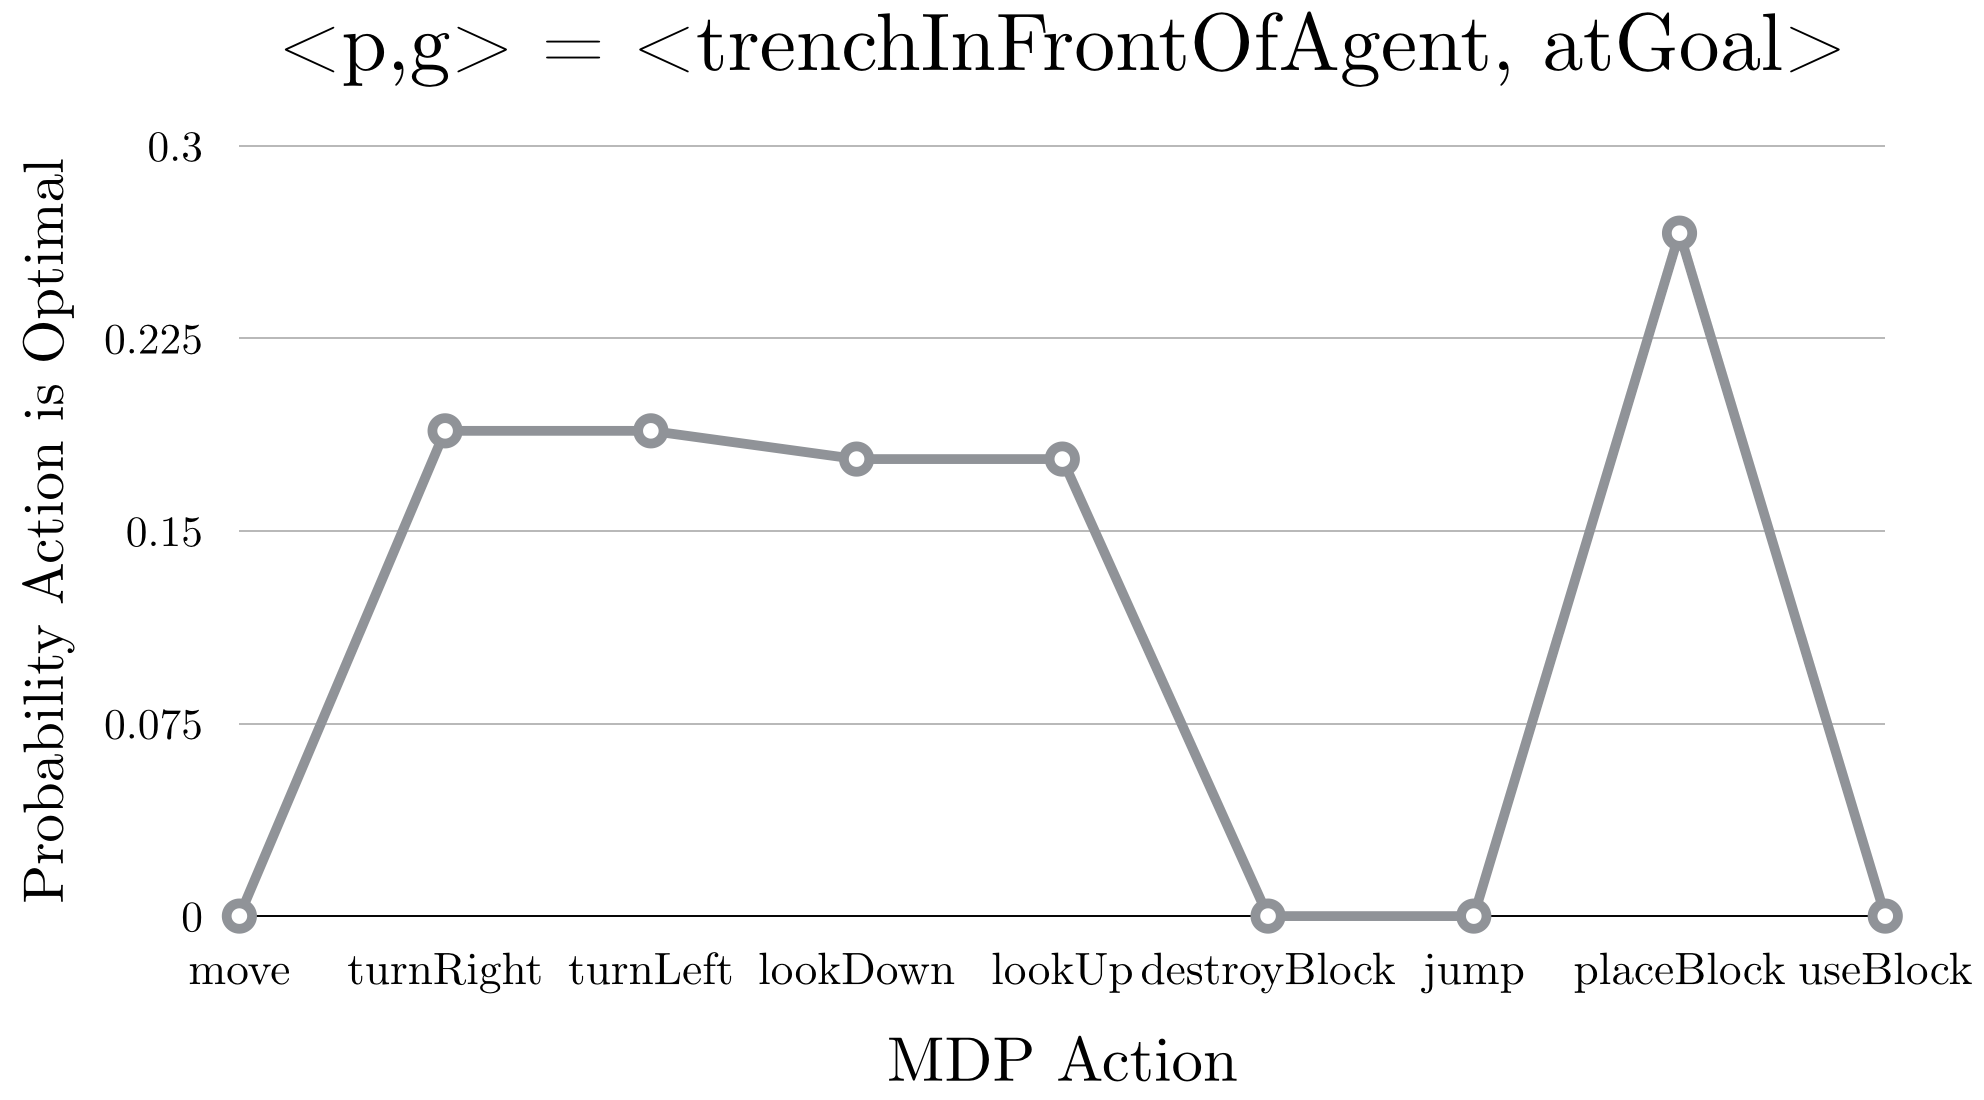
\includegraphics[scale=0.17]{figures/trench_aff.png}}
\label{fig:example_affs}
\caption{When the agent is looking toward the goal, it is generally better to move forward than do anything else. Alternatively, when the agent is faced with a trench, the agent should walk along the trench to look for gaps, or build a bridge across by looking down and placing blocks.}
\end{figure}

Here, $C(a_i)$ is the number of observed occurrences where $a_i$ was optimal across all worlds $W$,
$C(\bar{a_i})$ is the number of observed occurrences where $a_i$ was not optimal,
and $C(\phi_j, a_i)$ is the number of occurrences where $\phi_j=1$ and $a_i$ was optimal.
We determined optimality using the synthesized policy for each training world, $\pi_w$. More formally:

\begin{align}
C(a_i) &= \sum_{w \in W} \sum_{s \in w} (a_i \in \pi_w(s)) \\
C(\bar{a_i}) &= \sum_{w \in W} \sum_{s \in w} (a_i \not \in \pi_w(s) ) \\
C(\phi_j, a_i) &= \sum_{w \in W} \sum_{s \in w} (a_i  \in \pi_w(s) \wedge \phi_j == 1)
\end{align}

During the learning phase, the agent learns which actions are useful
under different conditions.  For example, consider the three different
problems shown in Figure~\ref{fig:minecraft}.  During training, we observe
that the \texttt{destroy} action is often optimal when the agent is
looking at a block of gold ore and the agent is trying to smelt gold
ingots.  Likewise, when the agent is not looking at a block of gold
ore in the smelting task we observe that the \texttt{destroy} action
is generally not optimal (i.e. destroying grass blocks is typically
irrelevant to smelting).  This information informs the distribution
over the optimality of the \texttt{destroy} action, which is used at
test time to encourage the agent to destroy blocks when trying to
smelt gold and looking at gold ore, but not in other situations
(unless another affordance suggests using \texttt{destroy}). Example
learned priors are shown in~\ref{fig:example_affs}.

At test time, the agent will see different, randomly generated worlds
from the same domain, and use the learned priors to increase its
speed at inferring a plan.  For simplicity, our learning process uses
a strict separation between training and test; after learning is
complete our model parameters remain fixed. 

%which actions were taken in each state. At test time, 
%when the agent is on a flat plane and needs to move to the gold ore, LRTDP will have learned
%that movement actions are useful (i.e. when the feature $\delta_j = (lookingAtGoldOre, smeltGold)$ is 0 (i.e. the agent is not looking
%at a block of gold ore or is trying to something other than smelt gold), then the probability
%that the destroy . Thus, the agent will apply the \texttt{destroyBlock}
%action when it is trying to smelt gold and is looking at gold.

% -- Subsection: Action Pruning --
\subsection{Affordance-Aware Planning}
\label{sec:action_pruning}
An {\em affordance-aware planner} uses affordances 
to prune actions from the action set under consideration 
by the planner on a state and
goal-specific basis. When a hard affordance model is used, defining
the action pruning method is trivial; when
$\Pr(a_i \in \mathcal{A}^*  \mid \phi_1, \ldots, \phi_n) = 0$
action $a_i$ is pruned from the planner's consideration. When
$\Pr(a_i \in \mathcal{A}^*  \mid \phi_1, \ldots, \phi_n) = 1$,
action $a_i$ remains in the action set to be searched by the planner.

When a non-deterministic affordance model, like Naive Bayes, is used,
a less restrictive approach must be taken. In this work,
we prune actions whose probability is below some threshold and
keep the rest. Empirically, we found the heuristic
of setting the threshold to $\frac{0.2}{|\mathcal{A}|}$ to
be effective (where $|\mathcal{A}|$ is the size
of the full action space of the OO-MDP). This threshold is
quite conservative and means that only actions
that are extremely unlikely to be optimal are pruned. 
In the future, we plan on exploring
stochastic action pruning methods with anytime planning
algorithms, but an advantage to this threshold pruning
approach is that it can be used in a large range of different
planning algorithms including A* (for deterministic domains),
Value Iteration, and Real-time
Dynamic Programming (RTDP)~\cite{barto95}. In this work, we present results 
using RTDP.

%% 1) Expert (discriminative or model)
%First, affordances may be specified by a domain expert.  The expert
%specifies a set of actions associated with a precondition-goal type
%pair. When the affordance is active, the actions suggested by the
%affordance are included in the agent's action set. For instance, if an
%agent is standing above a block of buried gold and is trying to smelt
%a block of gold, then an expert may indicate that the agent should
%consider the actions of looking down and digging.  All actions
%contributed by active affordances are grouped to yield the set of
%actions to consider for each state. Table~\ref{table:afford_kb_exp}
%shows several examples of expert-defined affordances.%

%% 2) Threshold
%Second, actions may be pruned by thresholding the posterior in
%Equation~\ref{eq:feature_rep}.  In this method, the affordances remove
%any actions whose probability of being optimal is below the provided
%threshold for each state. The threshold was determined empirically,
%and was set to $\frac{0.2}{|\mathcal{A}|}$, where $|\mathcal{A}|$ is
%the size of the full action space of the OO-MDP.  This threshold is
%quite conservative, and means that our approach only prunes actions
%which are extremely unlikely to be optimal.

% 3) Sampling
%% Lastly, actions may be pruned by sampling actions from the posterior,
%% treating each action's probability mass as a Bernouli trial and
%% sampling across the entire action set. In preliminary results, this
%% method did not perform as well as baselines - likely because the
%% weights associated with each action were too small. In future work, we
%% are interested in investigating more sophisticated approaches to
%% pruning actions with sampling.

%Through the use of any of the above methods, an affordance-aware
%planner prunes actions on a state-by-state basis, focusing the agent
%on relevant action possibilities of the environment, consequently
%reducing planning time. Any planner operating in an OO-MDP may be made
%affordance-aware with this approach.


% -- Table: Expert provided affordances --
\begin{table}[t]
\ra{1.15}
\small
\centering
\begin{tabular}{@{}lll}\toprule
Precondition & Goal Type & Actions \\ \midrule
\texttt{lookingTowardGoal} & \texttt{atLocation} & \texttt{\{move\}} \\
\texttt{lavaInFront} & \texttt{atLocation} & \texttt{\{rotate\}} \\
\texttt{lookingAtGold} & \texttt{hasGoldOre} & \texttt{\{destroy\}} \\
\bottomrule
\end{tabular}

\caption{Examples of expert-provided affordances.\label{table:afford_kb_exp}}
\end{table}


%As with human agents, multiple affordances often inform decision
%making at a given time.  Thus, affordance-aware planning agents
%operating within an OO-MDP will rarely make specific reference to
%particular affordances, but will instead reason about the world using
%the relevant action possibilities identified by the distribution in
%Equation~\ref{eq:final}.  That said, individual affordances can still
%be specified by experts, providing a natural spectrum between
%expert-provided knowledge and learned knowledge.

% ====== Section: Results ======
\section{Results}
\label{sec:results}

% Move average results HERE if want to go back to old method

We evaluate our approach using the game Minecraft and a collaborative
robotic cooking task.  Minecraft is a 3-D blocks game in which the
user can place, craft, and destroy blocks of different types.
Minecraft's physics and action space allow users to create complex
systems, including logic gates and functional scientific graphing
calculators\footnote{https://www.youtube.com/watch?v=wgJfVRhotlQ}.
Minecraft serves as a model for robotic tasks such as cooking
assistance, assembling items in a factory, object retrieval, and
complex terrain traversal.  As in these tasks, the agent operates in a
very large state-action space in an uncertain environment.
Figure~\ref{fig:minecraft} shows three example scenes from Minecraft
problems that we explore.  Additionally, we used expert-provided affordances to
enable a manipulator robot to infer helpful actions in response to a
person working on a kitchen task, shown in Figure~\ref{fig:baxter_results}.

% -- Subsection: Minecraft Tests --
\subsection{Minecraft}

% -- Table: Minecraft results --
\begin{table}
\ra{1.15}
\small
\begin{tabular}{@{}llll@{}}\toprule
Planner & Bellman & Reward & CPU \\ \midrule
&\hspace{-10mm}{\it Mining Task} \\
\texttt{RTDP} & 17142.1 ($\pm$3843) 		& {\bf -6.5} ($\pm$1)  & {\bf 17.6s}   ($\pm$4) \\
\texttt{EA-RTDP} 	& 14357.4 ($\pm$3275) 		& {\bf -6.5}   ($\pm$1) & 31.9s   ($\pm$8) \\
\texttt{LA-RTDP} 	& {\bf 12664.0} ($\pm$9340) 	& -12.7 ($\pm$5) & 33.1s   ($\pm$23) \\\hline
&\hspace{-10mm}{\it Smelting Task} \\
\texttt{RTDP} 	& 30995.0 ($\pm$6730) 		& {\bf -8.6}   ($\pm$1) & 45.1s   ($\pm$14) \\
\texttt{EA-RTDP} 	& 28544.0 ($\pm$5909) 		& {\bf -8.6}   ($\pm$1) & 72.6s   ($\pm$19) \\ 
\texttt{LA-RTDP} 	& {\bf 2821.9} 	 ($\pm$662) 	& -9.8   ($\pm$2) & {\bf 7.5s}  ($\pm$2) \\ \hline
&\hspace{-10mm}{\it Wall Traversal Task} \\
\texttt{RTDP} & 45041.7 ($\pm$11816) 		& -56.0   ($\pm$51) & {\bf 68.7s}   ($\pm$22) \\
\texttt{EA-RTDP} 	& 32552.0 ($\pm$10794) 		& -34.5   ($\pm$25) & 96.5s   ($\pm$39) \\ 
\texttt{LA-RTDP} 	& {\bf 24020.8} ($\pm$9239) 	& {\bf -15.8}   ($\pm$5) & 80.5s   ($\pm$34) \\ \hline
&\hspace{-10mm}{\it Trench Traversal Task} \\
\texttt{RTDP}  	& 16183.5 ($\pm$4509) 		& {\bf -8.1}   ($\pm$2) & 53.1s   ($\pm$22) \\
\texttt{EA-RTDP} 	& {\bf 8674.8} 	($\pm$2700) 	& -8.2   ($\pm$2) & {\bf 35.9s}   ($\pm$15) \\ 
\texttt{LA-RTDP} 	& 11758.4 ($\pm$2815) 		& -8.7   ($\pm$1) & 57.9s   ($\pm$20) \\ \hline
&\hspace{-10mm}{\it Plane Traversal Task} \\
\texttt{RTDP} & 52407 ($\pm$18432) 		& -82.6   ($\pm$42) & 877.0s   ($\pm$381) \\
\texttt{EA-RTDP} 	& 32928 ($\pm$14997) 		& -44.9   ($\pm$34) & 505.3s   ($\pm$304) \\
\texttt{LA-RTDP} 	& {\bf 19090} 	 ($\pm$9158) 	& {\bf-7.8}   ($\pm$1) & {\bf 246s}  ($\pm$159) \\
\bottomrule
\end{tabular}
\caption{RTDP vs. affordance-aware alternatives.}
\label{table:minecraft_results}
\end{table}

Our experiments consisted of five common tasks in Minecraft:
constructing bridges over trenches, smelting gold, tunneling through
walls, basic path planning, and digging to find an object. 

% TRAIN: NOTE ABOUT RANDOMLY GENERATED
The training set consists of 20 randomly generated instances of each task type, for a total of 100 instances. Each instance is extremely simply: 1,000-10,000 states (small enough to solve with tabular approaches). The output of our training process is the model parameter $\theta$, which informs our goal-based action prior. The full training process took approximately one hour run in parallel on a computing grid.

% TEST
The test set consisted of 20 randomly generated instances of the same task types, for a total of 100 instances. Each instance was extremely complex: 50,000-1,000,000 states (which is far too large to solve with tabular approaches).


%Figure~\ref{fig:learning_rate}
%shows the added effect of more training data.

%\begin{figure}
%\centering
%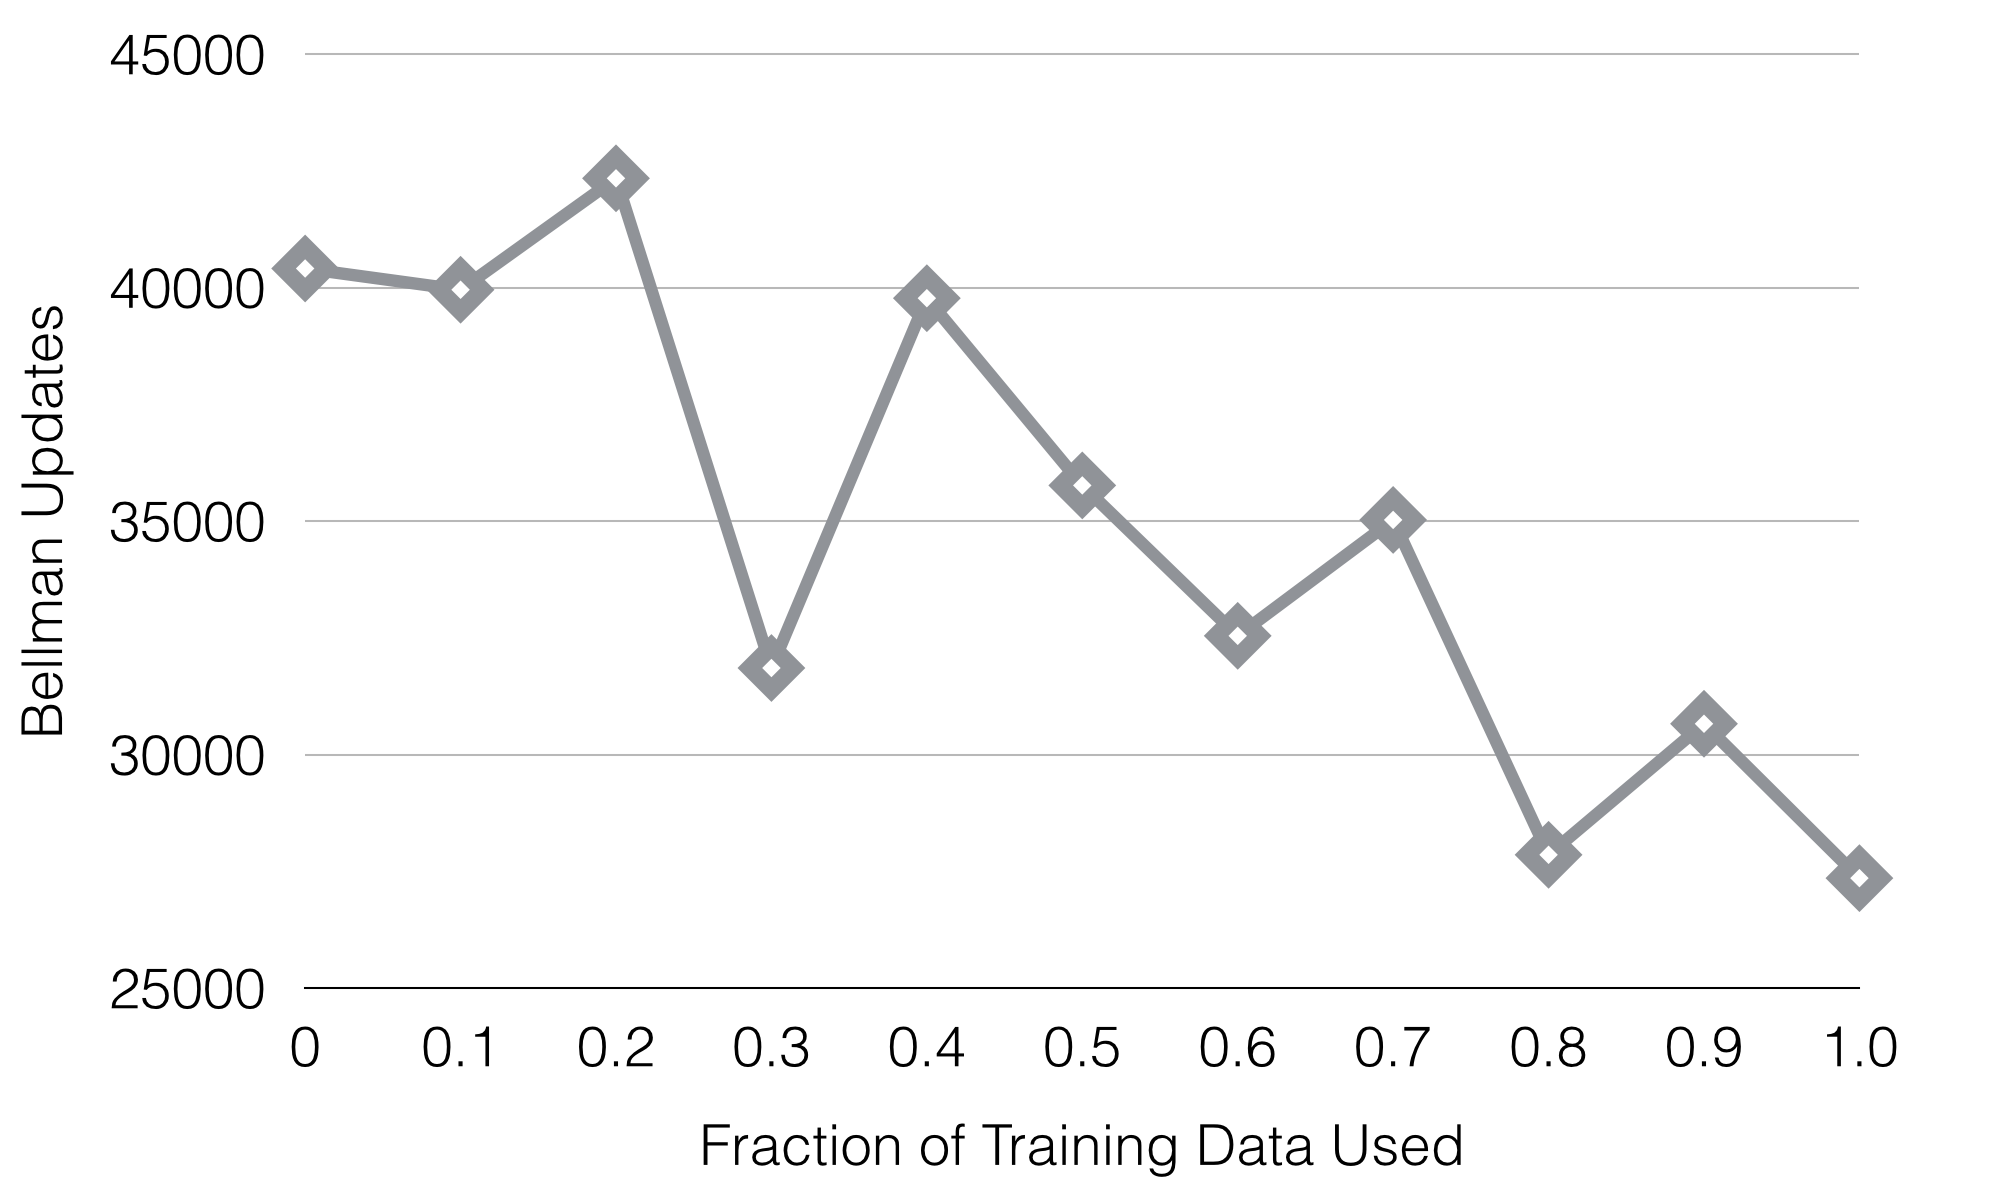
\includegraphics[width=1\linewidth]{figures/training_results.png}%
%\caption{The added effect of additional training data}
%\label{fig:learning_rate}
%\end{figure}

We fix the number of features at the start of training based on the
predicates defined by the OO-MDP, $|\mathcal{P}|$, and the goal types, $|G|$. We provided our system with a set of 51 features that were likely to aid in predicting the correct action across instances.

We use Real-Time Dynamic Programming (RTDP)~\cite{barto95} as our
baseline planner, a sampling-based algorithm that does not require the
planner to exhaustively explore states. We compare RTDP with learned
affordance-aware RTDP (LA-RTDP), and expert-defined affordance-aware
RTDP (EA-RTDP). We terminated each planner when the maximum change in
the value function was less than 0.01 for 100 consecutive policy
rollouts, or the planner failed to converge after 1000 rollouts.  The
reward function was $-1$ for all transitions, except transitions to
states in which the agent was in lava, where we set the reward to
$-10$. The goal was set to be terminal and the discount factor was
$\gamma = 0.99$.  To introduce non-determinism into our problem,
movement actions (move, rotate, jump) in all experiments had a small
probability (0.05) of incorrectly applying a different movement
action.  This noise factor approximates noise faced by a physical
robot that attempts to execute actions in a real-world domain and
can affect the optimal policy due to the existence of lava pits
that the agent can fall into. 

% -- Figure: Average results --
\begin{figure}[t]
%\begin{figure}
\centering
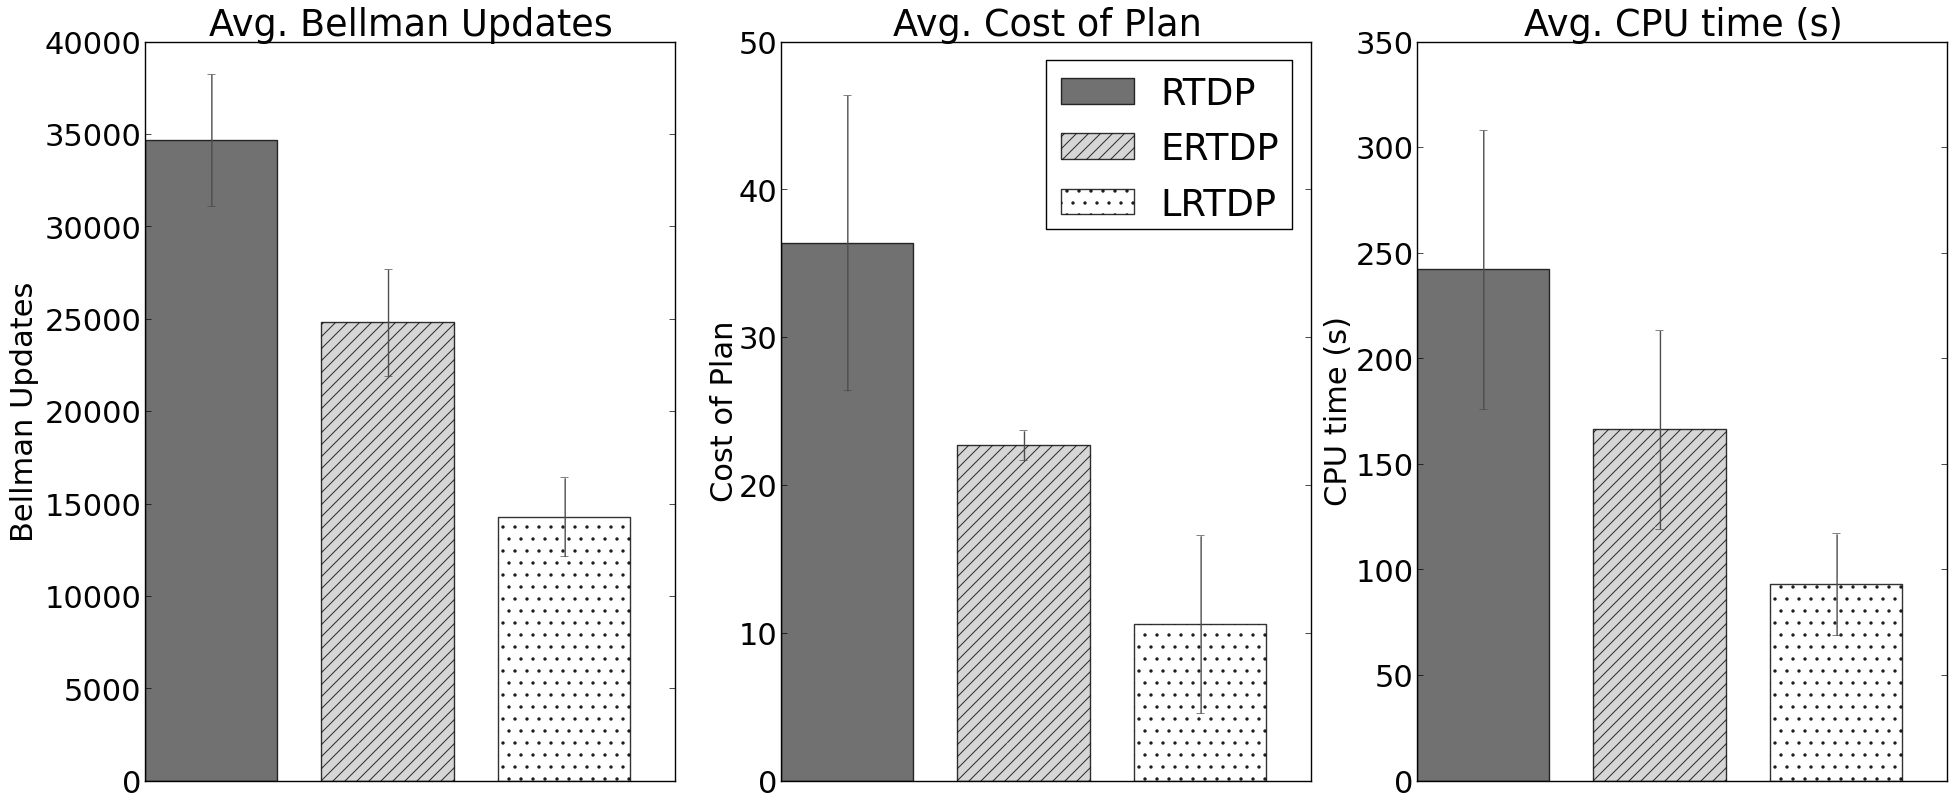
\includegraphics[width=1\linewidth]{figures/average_results_cropped.png}%
%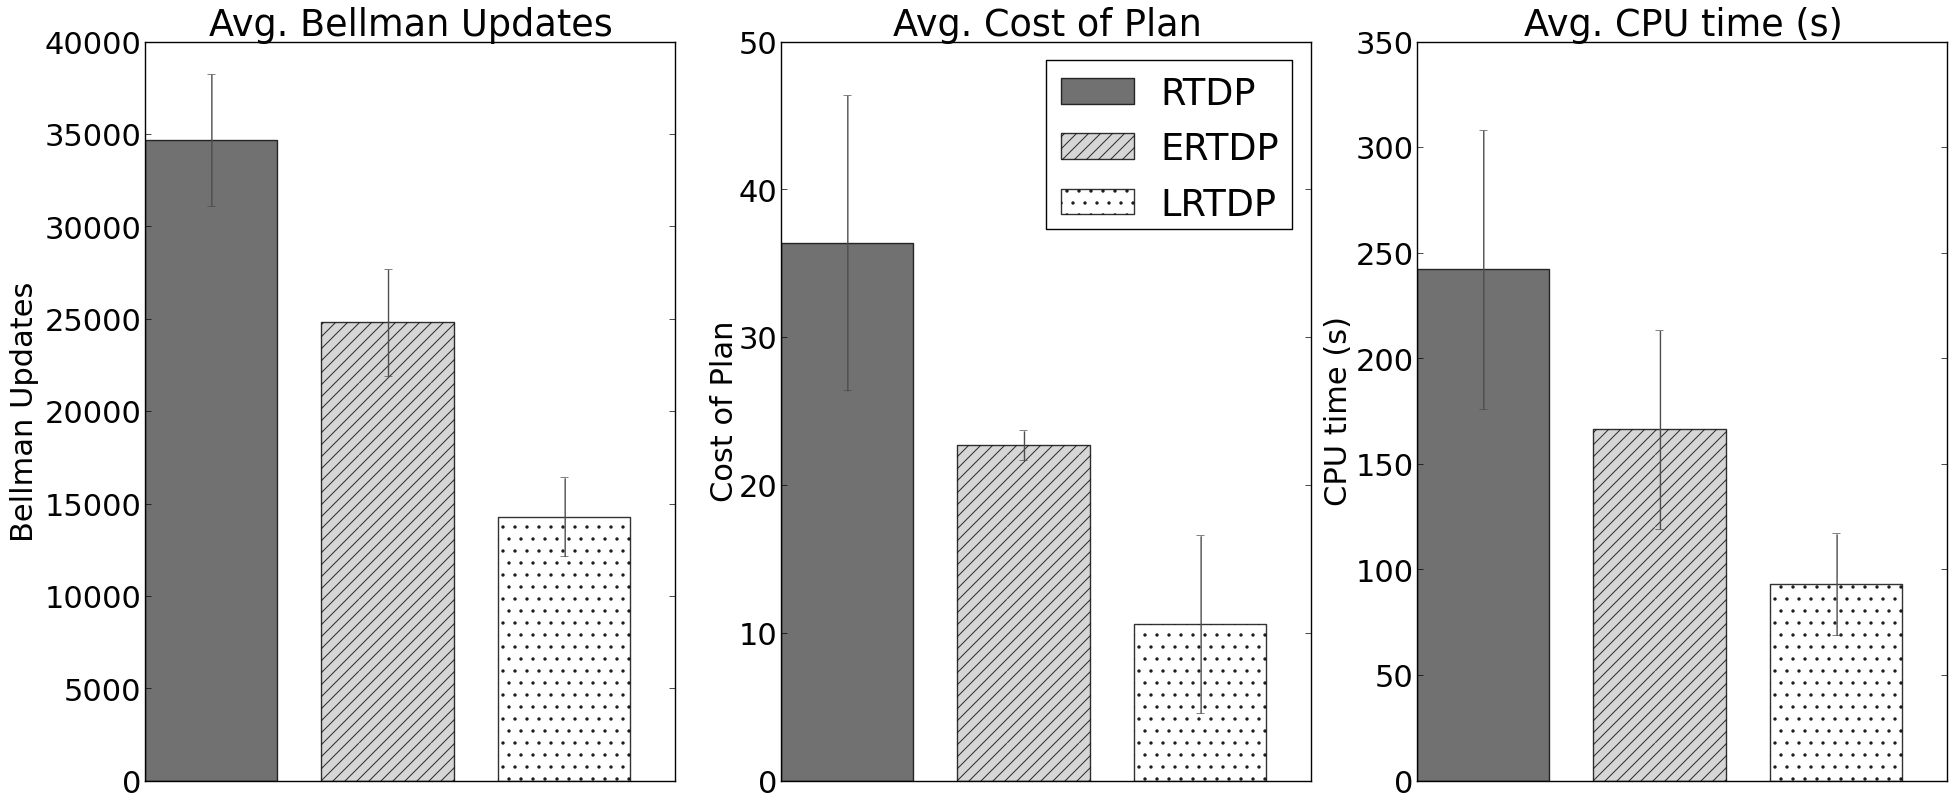
\includegraphics[scale=0.18]{figures/average_results_cropped.png}%
\caption{Average results from all maps.}
\label{fig:average_results}
\end{figure}
%\end{figure}

We report the number of Bellman updates executed by each planning
algorithm, the accumulated reward of the average plan, and the CPU
time taken to find a plan. Table~\ref{table:minecraft_results} shows
the average Bellman updates, accumulated reward, and CPU time for
RTDP, LA-RTDP and EA-RTDP after planning in 20 different maps of each
goal type (100 total). Figure~\ref{fig:average_results} shows the
results averaged across all maps.  We report CPU time for
completeness, but our results were run on a networked cluster where
each node had differing computer and memory resources. As a result,
the CPU results have some variance not consistent with the number of
Bellman updates in Table~\ref{table:minecraft_results}.  Despite this
noise, overall the average CPU time shows statistically significant
improvement overall with affordances, as shown in
Figure~\ref{fig:average_results}. Furthermore, we reevaluate each
predicate every time the agent visits a state, which could be optimized by caching predicate evaluations, further
reducing the CPU time taken for EA-RTDP and LA-RTDP.

Because the planners were forced to terminate after only 1000
rollouts, they did not always converge to the optimal policy. LA-RTDP on
average found a comparably better plan (10.6 cost) than EA-RTDP (22.7
cost) and RTDP (36.4 cost), found the plan in significantly fewer
Bellman updates (14287.5 to EA-RTDP's 24804.1 and RTDP's 34694.3) and in
less CPU time (93.1s to EA-RTDP's 166.4s and RTDP's 242.0s).  These
results indicate that while learned affordances gave the largest
improvements, expert-provided affordances can also significantly
enhance performance, and, depending on the domain, could add
significant value in making large state spaces tractable without the
overhead of supplying training worlds.


%Todo: Make this paragraph better
For some task types, LA-RTDP found a slightly worse plan on average than
RTDP ({\em e.g.} the mining task). This worse convergence is due to the fact that LA-RTDP
occasionally prunes actions that are in fact optimal (such as
pruning the \texttt{destroy} action in certain states of the mining task).
%To fix this, we could lower the threshold to allow for even more conservative action pruning. In future work, we plan on investigating approaches
%to dynamically adjusting the threshold based on planning feedback. 
Additionally, RTDP occasionally achieved a faster clock time because EA-RTDP and LA-RTDP also evaluate the affordance predicates in every state, adding a small amount of time to planning.

%\stnote{We need to explain the results in Table 3 about why
%  affordances don't always help.  Why is the reward sometimes worse
%  with affordances?  Why is the runtime sometimes worse? W hat is
%  special about the domains where that is happening?}


\begin{table}[b]
\ra{1.1}
\small
\begin{tabular}{@{}llll@{}}\toprule
Planner & Bellman & Reward & CPU \\ \midrule
\texttt{RTDP}   			&	27439 ($\pm$2348)		&	-22.6 ($\pm$9)		& 107 ($\pm$33) \\
\texttt{LA-RTDP} 			& 	{\bf 9935} ($\pm$1031)	&	{\bf -12.4} ($\pm$1)& {\bf 53} ($\pm$5) \\ \hline
\texttt{RTDP+Opt}  		&	26663 ($\pm$2298)		&	-17.4 ($\pm$4) 		& 129($\pm$35) \\
\texttt{LA-RTDP+Opt} 		& 	{\bf 9675} ($\pm$953)	&	{\bf -11.5} ($\pm$1)	&{\bf 93} ($\pm$10) \\ \hline
\texttt{RTDP+MA}  		&	31083 ($\pm$2468)		&	-21.7	 ($\pm$5)		&336 ($\pm$28) \\
\texttt{LA-RTDP+MA}  		& 	{\bf 9854} ($\pm$1034)	&	{\bf -11.7} ($\pm$1)	&{\bf 162} ($\pm$17) \\ %\hline
%\texttt{RTDP+MA+Opt}  	&	27143($\pm$2380)		&	-16.9($\pm$3.0)	&	323($\pm$38)		\\ 
%\texttt{LA-RTDP+MA+Opt} & 	{\bf 10622($\pm$1046)}	&	{\bf -13.4($\pm$1.0)}	&	{\bf 237($\pm$29)}		\\
\bottomrule
\end{tabular}
\caption{Affordances with Temporally Extended Actions}
\label{table:temp_ext_act_results}
\end{table}


% -- Subsection: Temporally Extended Actions --
\subsection{Temporally Extended Actions and Affordances}

We compared our approach to Temporally Extended Actions: macro-actions
and options. We conducted these experiments with the same
configurations as our Minecraft experiments. Domain experts provided
the option policies and macro-actions.

Table~\ref{table:temp_ext_act_results} indicates the results of
comparing RTDP equipped with macro-actions, options, and affordances
across 100 different executions in the same randomly generated
Minecraft worlds. The results are averaged across tasks of each type
presented in Table~\ref{table:minecraft_results}. Both macro-actions
and options add a significant amount of time to planning due to the
fact that the options and macro-actions are being reused in
multiple MDPs that each require recomputing the resulting transition
dynamics and expected cumulative reward when applying each
option/macro-action (a cost that is typically amortized in classic
options work where the same MDP state space and transition dynamics
are used). This computational cost might be reduced when using a Monte
Carlo planning algorithm that does not need the full transition
dynamics and expected cumulative reward.  Furthermore, the branching
factor of the state-action space significantly increases with
additional actions, causing the planner to run for longer and perform
more Bellman updates.  Despite these extra costs in planning time,
earned reward with options was higher than without, demonstrating that
our expert-provided options add value to the system.

With affordances, the planner found a better plan in less CPU time,
and with fewer Bellman updates. These results support the claim that
affordances can handle the augmented action space provided by
temporally extended actions by pruning away unnecessary actions, and
that options and affordances provide complementary information.

% -- Subsection: Baxter --
\subsection{Cooking Robot}

To assess affordances applied to a real-world robotic task, we created
a cooking domain that requires the robot to choose helpful actions for
a person following a recipe. The human participant and the robotic companion are each modeled as separate
OO-MDPs. From the robot?s perspective, the human is just a stochastic element of its OO-MDP's
transition dynamics.

There were three spaces: human counter, robot counter, sink.  We had
four ingredient bowls, two mixing bowls, and two tools that could be
in any of the three spaces, in any configuration.  There were four
ingredients: cocoa powder, sugar, eggs, and flour.  Each
container/tool could be on one of three spaces, and each ingredient in
one of the containers in an either mixed or unmixed state.  (e.g., the
state of all the ingredients in a mixing bowl is different than the
state of the drys mixed with the wets mixed individually in a bowl.)
Although this fine-grained state space is much larger than needed for
any one recipe, it enables support for a variety of different recipes,
ranging from brownies to mashed potatoes.  Because of its
fine-grained nature, our cooking state space has
$\num[round-precision=3, round-mode=figures]{47258883}$ states when
configured with the ingredients and tools necessary to make brownies.

\begin{table}[t]
\ra{1.1}
\small
\begin{tabular}{@{}llll@{}}\toprule
Planner & Bellman & Reward & CPU \\ \midrule
&\hspace{-10mm}{\it Dry Ingredients} \\
\texttt{RTDP} 	& 20000 ($\pm$0) 			& {-123.1} ($\pm$0)  & {56.0s}   ($\pm$2.9) \\
\texttt{EA-RTDP} 	& {\bf 2457.2} ($\pm$53.2) 		& {\bf -6.5}   ($\pm$0) & {\bf 10.1s}   ($\pm$0.3) \\  \hline
&\hspace{-10mm}{\it Wet Ingredients} \\
\texttt{RTDP} 	& 19964 ($\pm$14.1) 			& { -123.0}   ($\pm$0) & 66.6s   ($\pm$9.9) \\
\texttt{EA-RTDP} 	& {\bf 5873.5} ($\pm$53.7) 		& {\bf -6.5}   ($\pm$0) & {\bf 15.6s}   ($\pm$1.2) \\ \hline
&\hspace{-10mm}{\it Brownie Batter} \\
\texttt{RTDP} 	& 20000 ($\pm$0) 			& -123.4   ($\pm$0.7) & { 53.3s}   ($\pm$2.4) \\
\texttt{EA-RTDP} 	& {\bf 6642.4} ($\pm$36.4) 		& {\bf -7.0}   ($\pm$0) & {\bf 31.9s}   ($\pm$0.4) \\ 
\bottomrule
\end{tabular}
\caption{RTDP vs. EA-RTDP for robotic kitchen tasks}
\label{table:baxter_results}
\end{table}



%To remove a large number of self-transitions, we provided affordances for each
%action. For example, one affordance specified that mixing should only occur 
%in containers that contain ingredients. An affordance for pouring required 
%the container being poured to contain ingredients. 

% -- Figure: Baxter results/image
\begin{figure}[b]
\centering
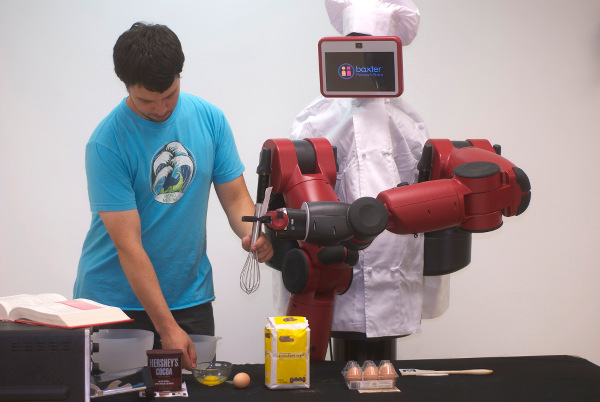
\includegraphics[width=0.75\linewidth]{figures/baxter_scaled.jpg}%
  \caption{Affordances enable a robot to efficiently infer helpful actions in
    very large state spaces, such as a kitchen.}
  \label{fig:baxter_results}
\end{figure}

We divided a brownie recipe into three subgoals: combining and mixing
the dry ingredients, combining and mixing the wet ingredients, and
combining these two mixtures into a batter. For each subgoal, we
provided affordances specific to the objects used in that subgoal; for
example, a whisk should only be used to mix wet ingredients.  We used
EA-RTDP to search for the least-cost plan to complete the recipe.  The
robot inferred actions such as handing off the whisk to the person to
mix the wet ingredients.


In Table~\ref{table:baxter_results} we compare between standard RTDP
and EA-RTDP planning for each of the three subgoals. Because the
state-action space is reduced significantly, EA-RTDP can plan
successfully in a short amount of time. Standard RTDP always
encountered the maximum number of rollouts specified at the maximum
depth each time, even with a relatively small number of objects.
(Unlike our previous CPU time results, these results took place on the
same multi-core computer.)

We provide a video\footnote{Watch at https://vimeo.com/106226282} 
showing how this affordance-aware planner running
on a robot can help a person cook by dynamically replanning through
constant observations. After observing the placement of a cocoa
container in the robot's workspace, the robot fetches a wooden spoon
to allow the person to mix. After observing an egg container, the
robot fetches a whisk to help beat the eggs. 
%Because we modeled the
%culinary world as an MDP and replanned at every observation, the robot
%dynamically resolves failures and accounts for unpredictable user
%actions.
The robot dynamically resolves failures and accounts for unpredictable
user actions; in the video, the robot fails to grasp the wooden spoon on
the first attempt and must retry the grasp after it observed no state
change.


\section{Related Work}
\label{sec:related-work}

In this section, we discuss the differences between affordance-aware
planning and other forms of knowledge engineering that have been used
to accelerate planning.  This paper builds on previous work\footnote{A
  previous version of the proposed approach may be seen planning in
  Minecraft at https://vimeo.com/88689171} published at two workshops
(redacted for review).

% -- Subsection: Stochastic --
\subsection{Stochastic Approaches}

Temporally extended actions are actions that the agent can select like
any other action of the domain, except executing them results in
multiple primitive actions being executed in succession. Two common
forms of temporally extended actions are {\em
  macro-actions}~\cite{hauskrecht98} ~and {\em
  options}~\cite{sutton99}.  Macro-actions are actions that always
execute the same sequence of primitive actions. Options are defined
with high-level policies that accomplish specific sub tasks. For
instance, when an agent is near a door, the agent can engage the
`door-opening-option-policy', which switches from the standard
high-level planner to running a policy that is crafted to open doors.
Although the classic options framework is not generalizable to
different state spaces, creating {\em portable} options is a topic of
active
research~\cite{konidaris07,konidaris2009efficient,Ravindran03analgebraic,croonenborghs2008learning,andre2002state,konidaris2012transfer}.

Since temporally extended actions may negatively impact planning
time~\cite{Jong:2008zr} by adding to the number of actions the agent
can choose from in a given state, combining affordances with
temporally extended actions allows for even further speedups in
planning, as demonstrated in Table~\ref{table:temp_ext_act_results}. In
other words, affordances are complementary knowledge to options and
macro-actions.

% --- Action Pruning ---
Sherstov and Stone~\cite{sherstov2005improving} considered MDPs for
which the action set of the optimal policy of a source task could be
transferred to a new, but similar, target task to reduce the learning
time required to find the optimal policy in the target task.
Affordances prune away actions on a state-by-state basis, enabling
more aggressive pruning whereas the learned action pruning is on per-task
level.

Rosman and Ramamoorthy~\cite{rosman2012good} provide a method for
learning action priors over a set of related tasks. Specifically, they
compute a Dirichlet distribution over actions by extracting the
frequency that each action was optimal in each state for each
previously solved task.  Action priors can only be used with
planning/learning algorithms that work well with an $\epsilon$-greedy
rollout policy, while affordances can be applied to almost any MDP
solver.  Action priors are only active for a fraction $\epsilon$ of
the time steps, which is quite small, limiting the improvement they
can make to the planning speed.  Finally, as variance in tasks
explored increases, the priors will become more uniform. In contrast,
affordance-aware planning can handle a wide variety of tasks in a
single knowledge base, as demonstrated by
Table~\ref{table:minecraft_results}.

% --- Heuristics ---
Heuristics in MDPs are used to convey information about the value of a
given state-action pair with respect to the task being solved and
typically take the form of either value function
initialization~\citep{Hansen:1999qf}, or reward shaping\cite{potshap}.
However, heuristics are highly dependent on the reward function and
state space of the task being solved, whereas affordances are state
space independent and may be learned easily for different reward
functions. If a heuristic can be provided, the combination of
heuristics and affordances may even more greatly accelerate planning
algorithms than either approach alone.

% -- KnowRob --
Previous approaches, such as KnowRob~\citep{tenorth2012knowledge,tenorth2009knowrob} have developed complex reasoning systems designed to integrate existing forms of knowledge from a variety of sources for use in robotics applications. These systems emphasize knowledge representation and processing rather than planning. KnowRob, in particular, works ``by exploiting existing sources of knowledge as much as possible?, as opposed to learning through simulation.

% -- Subsection: Deterministic knowledge engineering approaches --
\subsection{Deterministic Approaches}

There have been several attempts at engineering knowledge
to decrease planning time for deterministic planners. These are
fundamentally solving a different problem from what we are interested
in since they deal with non-stochastic problems, but there are
interesting parallels nonetheless.

% --- Hierarchical Task Networks ---

Hierarchical Task Networks (HTNs) employ \textit{task decompositions}
to aid in planning~\cite{erol1994htn}. The agent decomposes the goal
into smaller tasks which are in turn decomposed into smaller
tasks. This decomposition continues until immediately achievable
primitive tasks are derived. The current state of the task
decomposition, in turn, informs constraints which reduce the space
over which the planner searches. At a high level HTNs and affordances
both achieve action pruning by exploiting some form of supplied
knowledge. We speculate that the additional action pruning provided by our affordances
is complementary to the pruning offered by HTNs.

One significant difference between HTNs and our planning system is that HTNs do not incorporate reward into their planning. Consequently, they lack any guarantees of the quality of any
induced plan. Additionally, the degree of supplied knowledge in HTNs
far exceeds that of affordances: HTNs require not only constraints for
sub-tasks but a hierarchical framework of arbitrary
complexity. Affordances require either simple symbolic knowledge, as
illustrated in Table ~\ref{table:afford_kb_exp}, or a set of
predicates for use as features and a means of generating candidate
state spaces.

% --- pHTN ---

An extension to the HTN is the probabilistic Hierarchical Task Network (pHTN)~\cite{li2010learning}. In pHTNs, the underlying physics of the primitive actions are deterministic. The goal of pHTN planning is to find a sequence of deterministic primitive actions that satisfy the task, with the addition of matching user preferences for plans, which are expressed as probabilities for using different HTN methods. As a consequence, the probabilities in pHTNs are with regard to probabilistic search rather than planning in stochastic domains, as we do.

% --- Temporal Logic ---

Bacchus and
Kabanza~\cite{Bacchus95usingtemporal,Bacchus99usingtemporal} provided
planners with domain dependent knowledge in the form of a first-order
version of linear temporal logic (LTL), which they used for control of
a forward-chaining planner. With this methodology, a \textsc{Strips}
style planner may be guided through the search space by pruning
candidate plans that falsify the given knowledge base of LTL formulas,
often achieving polynomial time planning in exponential space.  LTL
formulas are difficult to learn, placing dependence on an expert,
while we demonstrate that affordances can be automatically learned
from experience.

Our approach is related to preferred actions used by
LAMA~\citep{richter10} in that our agent learns actions which are
useful for a specific problem and expands those actions first.
However our approach differs in that it generalizes this knowledge
across different planning problems, so that the preferred actions in
one problem influence search in subsequent problems in the domain.

% -- OO-MDPs --
\subsection{Models}
Our planning approach relies critically on the the ability of the OO-MDP to express properties of objects in a state, which is shared by other models such as First-Order MDPs (FOMDPs). As a consequence, a domain that can be well expressed by a FOMDP may also benefit from our planning approach. However FOMDPs are purely symbolic, while OO-MDPs can represent states with objects defined by numeric, relational, categorical, and string attributes. Moreover, OO-MDPs enable predicates to be defined that are evaluative of the state rather than attributes that define the state, which makes it easy to add high-level information without adding complexity to the state definition and transition dynamics to account for them. These abilities make OO-MDPs better-suited for the kind of robotic tasks in which we are interested, since it is common to have different objects with spatial properties that are best expressed with numeric values.


% ====== Section: Conclusion ======
\section{Conclusion}
\label{sec:conclusion}
We proposed a novel approach to representing transferable planning
knowledge in terms of {\em affordances}~\cite{gibson77}. Affordances
allow an agent to efficiently prune actions based on learned or expert
provided knowledge, significantly reducing the number of state-action
pairs the agent needs to evaluate in order to act near optimally. We
demonstrated the effectiveness of the affordance model by comparing
RTDP to its affordance-aware equivalents in a series of challenging
planning tasks in the Minecraft domain. Further, we designed a
learning process that allows an agent to autonomously learn useful
affordances that may be used across a variety of task types, reward
functions, and state spaces, allowing for convenient extensions to
robotic applications.  Additionally, we compared the effectiveness of
augmenting planners with affordances with temporally extended actions,
and the combination of the two. The results suggest that affordances
may be combined with temporally extended actions to provide
improvements in planning.  Lastly, we deployed an affordance-aware
planner on a robot in a collaborative cooking task.

In the future, we hope to automatically discover useful state space
specific subgoals online---a topic of some active research
\cite{Mcgovern01automaticdiscovery,Simsek:2005:IUS:1102351.1102454}.
Automatic discovery of subgoals would allow affordance-aware planners
to take advantage of the goal-oriented focus of affordances, and would
further reduce the size of the explored state-action space by
improving the effectiveness of action pruning. Finally we are excited
to explore learning affordances from other sources besides learning
from policies.  For example, learning from human feedback via
imitation learning or reinforcement learning could allow our agent to
bias its actions in promising directions by following a person's
example.  Another promising direction is to explore continuous
learning.  In this mode, the agent uses affordances as it learns,
allowing it to build a knowledge base that expands as it goes.

Additionally, we hope to explore methods that capitalize on
the distribution over optimal actions, such as incorporating
affordances with a forward search sparse sampling
algorithm~\cite{walsh2010integrating}, or replacing the Naive Bayes
model with a more sophisticated model, such as Logistic Regression or
a Noisy-OR.  We are also investigating methods to stochastically prune
actions rather than requiring a hard threshold parameter to be defined
(or estimated).  These methods will enable agents to acquire and
leverage general planning knowledge to infer actions in very large
state spaces.



{\small
\bibliographystyle{plainnat}
\bibliography{main}
}
\end{document}


